% %% %%%%%%%%%%%%%%%%%%%%%%%%%%%%%%%%%%%%%%%%%%%%%%%%%%%%%%%%%%
% steps.tex
%
% Author:  Mauricio Matamoros
% License: MIT
%
% %% %%%%%%%%%%%%%%%%%%%%%%%%%%%%%%%%%%%%%%%%%%%%%%%%%%%%%%%%%%

%!TEX ROOT=../main.tex
%!TEX ROOT=../references.bib

% CHKTEX-FILE 1
% CHKTEX-FILE 46

\cleardoublepage
\section{Instrucciones}%
\label{sec:instructions}
\begin{enumerate}[noitemsep]
	\item Descargue y pruebe la tarjeta simuladora siguiendo los pasos de la \cref{sec:step1}.

	\item Revise cuidadosamente las \cref{sec:step1,sec:step2,sec:step3,sec:step4}.

	\item Calcule las resistencias para un divisor de voltaje óptimo para el circuito simulado siguiendo las instrucciones de la \cref{sec:step2}.

	\item Con base en el voltaje de referencia, calcule el factor de conversión de valores discretos a centígrados tal como lo indica la \cref{sec:step3}.

	\item Tomando como base el programa de ejemplo del \Cref{sec:temperature-py}
	y lo aprendido en las \cref{sec:step1,sec:step2,sec:step3,sec:step4}
	realice el programa descrito en la \cref{sec:programs} y, con los resultados obtenidos, responda el cuestionario de la \cref{sec:questionnaire}.
\end{enumerate}

% %% %%%%%%%%%%%%%%%%%%%%%%%%%%%%%%%%%%%%%%%%%%%%%%%%%%%%%%%%%%
% step-1.tex
%
% Author:  Mauricio Matamoros
% License: MIT
%
% %% %%%%%%%%%%%%%%%%%%%%%%%%%%%%%%%%%%%%%%%%%%%%%%%%%%%%%%%%%%


%!TEX ROOT=../main.tex
%!TEX ROOT=../references.bib

% CHKTEX-FILE 1
% CHKTEX-FILE 46

\subsection{Paso 1: Configuración del Simulador}%
\label{sec:step1}

Descargue el simulador de \url{https://github.com/kyordhel/RPiVirtualBoards} ejecutando la siguiente línea de comandos:

\begin{Verbatim}[fontsize=\footnotesize]
git clone https://github.com/kyordhel/RPiVirtualBoards.git
cd RPiVirtualBoards
\end{Verbatim}

A continuación instale todas las dependencias requeridas por el simulador usando \emph{pipenv}\footnotemark{}:

\begin{Verbatim}[fontsize=\footnotesize]
pipenv install
\end{Verbatim}

Finalmente, pruebe el simulador ejecutando la siguiente línea:

\begin{Verbatim}[fontsize=\footnotesize]
pipenv run python temperature.py
\end{Verbatim}

Si, por otro lado, no desea mantener el simulador conmo un proyecto aislado, puede instalar los paquetes con \emph{pip} después de clonar el proyecto:

\begin{Verbatim}[fontsize=\footnotesize]
pip install  --user -r requirements.txt
./temperature.py
\end{Verbatim}

Si la configuración es correcta, verá una ventana similar a la de la \Cref{fig:simboard} con los valores de temperatura simulados cambiando.

\begin{figure}[H]
	\centering%
	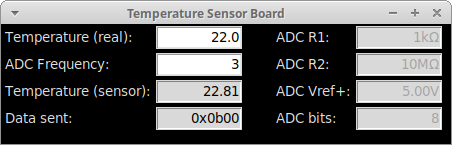
\includegraphics[width=0.5\textwidth,height=8cm,keepaspectratio]{img/simboard.png} %CHKTEX 8
	\caption{Simulador de tarjeta lectora de LM35 con DAC \IIC}%
	\label{fig:simboard} %CHKTEX 24
\end{figure}

\footnotetext{\emph{pipenv} es una herramienta que facilita la creación y administración de entornos virtuales en cualquier proyecto escritos en Python, llevando un control riguroso de los paquetes de los que depende dicho proyecto. Se puede instalar fácilmente con la línea \texttt{pip install --user pipenv}}
% %% %%%%%%%%%%%%%%%%%%%%%%%%%%%%%%%%%%%%%%%%%%%%%%%%%%%%%%%%%%
% step-2.tex
%
% Author:  Mauricio Matamoros
% License: MIT
%
% %% %%%%%%%%%%%%%%%%%%%%%%%%%%%%%%%%%%%%%%%%%%%%%%%%%%%%%%%%%%

% CHKTEX-FILE 1
% CHKTEX-FILE 46
%!TEX ROOT=../main.tex
%!TEX ROOT=../references.bib

\subsection{Paso 2: Cálculo del divisor de voltaje}%
\label{sec:step2}

El simulador configurado en la \Cref{sec:step1} implementa la simulación de un sensor de temperatura LM35 en configuración básica acoplado a un circuito ADC con un divisor de voltaje en $V_{Ref+}$ y $V_{Ref-}$ a tierra, mismo que se configura con la línea:

\lstinputlisting[%
	firstline=58,
	lastline=58,
	label={lst:adc-board-config},
	caption=Configuración del ADC del sensor LM35 virtual \IIC{} (\texttt{temperature.py:58})
]{src/temperature.py}

La función \texttt{run\_temperature\_board} recibe tres parámetros, los valores de las resistencias $R_1$ y $R_2$ para la alimentación del $V_{Ref+}$ y un boleano que configura el módulo ADC para operar con una presición de 8 bits (\texttt{p8bits=True}) o de 10 bits  (\texttt{p8bits=False}).

Sin embargo, los valores por defecto de las resistencias usadas no son óptimos, ya que hacen que el módulo ADC opere en rango completo de $0-5V$ mientras que el LM35 en configuración básica opera en el rango de $0.02-1.50V$, motivo por el cual deben proporcionarse otros valores para las resistencias.

Para calcular las resistencias del divisor de voltaje, lea cuidadosamente la \Cref{sec:intro-adc} y utilice la \Cref{eqn:vdiv} tomando un valor fijo para $R_1$ (ej.~$10k\Omega$) y despejando $R_2$.

\begin{importantbox}{\bfseries IMPORTANTE}
Verifique que al calcular los valores de $R_1$ y $R_2$ aproxima sus resultados a los valores de resistencias comerciales, por ejemplo cambiando una resitencia de $1273.5\Omega$ por una resistencia comercial de $1k2$.
\end{importantbox}
% %% %%%%%%%%%%%%%%%%%%%%%%%%%%%%%%%%%%%%%%%%%%%%%%%%%%%%%%%%%%
% step-3.tex
%
% Author:  Mauricio Matamoros
% License: MIT
%
% %% %%%%%%%%%%%%%%%%%%%%%%%%%%%%%%%%%%%%%%%%%%%%%%%%%%%%%%%%%%

%!TEX ROOT=../main.tex
%!TEX ROOT=../references.bib

% CHKTEX-FILE 1
% CHKTEX-FILE 46

\subsection{Paso 3: Lectura del sensor LM35}%
\label{sec:step3}

Para leer la temperatura se necesita convertir los valores discretos leídos por el ADC en valores de temperatura.
Esto se puede realizar mediante un simple análisis debido a la linearidad del LM35.
En un ADC típico se obtienen dos lecturas: V\textsubscript{OUT+} y V\textsubscript{OUT-}, de las cuales la segunda es la referencia del LM35 y por lo tanto, la diferencia entre estos voltajes será proporcional a la temperatura en escala centígrada.
Esto expresado matemáticamente es:

\begin{equation*}
	T[^{o}C] \propto V_{diff} = V_{OUT+}-V_{OUT-}
\end{equation*}

\noindent o bien

\begin{equation*}
	T[^{o}C] = k \times V_{diff} = k \times \big( V_{OUT+}-V_{OUT-} \big)
\end{equation*}

\noindent lo que implica que en $T = 0^{o}C; V_{OUT+}=V_{OUT-} \rightarrow V_{diff} = 0$

\medskip
Es necesario entonces calcular la constante de proporcionalidad $k$.
Sabemos que el ADC entregará lecturas de 0 a 1024 para los voltajes registradoes entre \GND y \textsc{Aref}.
Por ejemplo, con el LM35 en una configuración básica ($V_{OUT-}$ en \GND), $V_{Ref+} = 2.72V$ y considerando que que $1^{o}C = 0.01V$ se tendría:
\begin{align*}
	T[^{o}C] &= V_{diff} \times \frac{2.72[V]}{ 1024 \times 0.01[\tfrac{V}{^{o}C}] }  \\
	         &= V_{diff} \times \frac{2.72}{ 10.24 }[^{o}C]  \\
	         &= 0.266 V_{diff}[^{o}C]  \\
\end{align*}

\noindent o bien, generalizando para todo voltaje de referencia:
\begin{equation*}
	T[^{o}C] = V_{diff} \times \frac{V_{Ref+}}{ 10.24 }[^{o}C]
\end{equation*}

Esta fórmula de conversión, o su equivalente según el divisor de voltaje utilizado, deberá programarse en la Raspberry Pi que adquiera los valores discretos de temperatura del sensor.

% %% %%%%%%%%%%%%%%%%%%%%%%%%%%%%%%%%%%%%%%%%%%%%%%%%%%%%%%%%%%
% step-4.tex
%
% Author:  Mauricio Matamoros
% License: MIT
%
% %% %%%%%%%%%%%%%%%%%%%%%%%%%%%%%%%%%%%%%%%%%%%%%%%%%%%%%%%%%%

%!TEX ROOT=../main.tex
%!TEX ROOT=../references.bib

% CHKTEX-FILE 1
% CHKTEX-FILE 46

\subsection{Paso 4: Adquisición de datos via \IIC}%
\label{sec:step4}

Una forma de leer del puerto serial \IIC{} de la Raspberry Pi usando Python es mediante el paquete \texttt{smbus}, o su sucesor \texttt{smbus2} que incorpora exactamente las mismas funciones pero está implementada completamente en Python en lugar de ser un envoltorio para la \emph{SMBusLib} de C.

El primer paso es instanciar un objeto de tipo \texttt{SMBus} indicando el número de dispositivo a controlar (véase el \Cref{lst:iic-read}, línea 1).

\lstinputlisting[%
	linerange={30-32,34-40}, %CHKTEX 8
	label={lst:iic-read},%
	caption={Lectura de datos usando \IIC{} (\texttt{temperature.py:30--43})}
]{src/temperature.py}

Debido a que las transmisiones de datos en \IIC{} son síncronas y completamente controladas por el dispositivo maestro, no es necesario realizar complicadas rutinas que almacenen datos en búfferes y controlen interrupciones.
En su lugar, simplemente se genera un mensaje \IIC{} de tipo lectura o escritura y se realiza la transacción con la función \texttt{i2c\_rdwr} (en \IIC{} toda lectura requiere de una escritura al canal SDA).
Para generar el mensaje es necesario especificar tanto la dirección del dispositivo esclavo colmo los datos a enviar, en el caso de una escritura, o el número de bytes que se leerán de éste.
Esta operación se muestra en el \Cref{lst:iic-read}, líneas 5 y 6.

Un aspecto a tomar en cuenta es que las transmisiones seriales de datos no son otra cosa que flujos de bytes sin significado alguno, mientras que las variables en Python son objetos con un tipo inferido sobre los cuales se pueden realizar un gran número de operaciones; es decir, ambos son incompatibles.
Es por esto que es necesario convertir los datos binarios en algo que Python pueda entender.
Estas conversiones las realizan las funciones \texttt{pack} y \texttt{unpack} del paquete \texttt{struct}.
En particular, la función \texttt{unpack} recibe un \textit{bytearray} y un especificador de formato que indica cómo deben interpretarse los bytes en el arreglo para poder generar una tupla de $n$ elementos interpretados.

En el \Cref{lst:iic-read} (línea 8), se realiza la lectura de 1 byte como entero no signado (ADC de 8 bits con rango de 0--255), por lo que se utiliza el especificador de formato \texttt{`<B'} para leer 1 byte no signado (\texttt{unsigned char} en C).
Si se quisieran leer 16 bits (ADC de 10 bits) habrpia que especificar un \emph{unsigned half int} con la cadena de formato \texttt{`<H'}. El caracter de \emph{menor que} ($<$) en la cadena de formato se requiere para especificar que los bytes están codificados en \emph{little endian}, es decir, con el byte menos significativo a la izquierda, que es la codificación por defecto en \IIC{}.

